
\documentclass[sigconf]{acmart}

\usepackage{tikz}
\usetikzlibrary{arrows.meta,positioning}

\bibliographystyle{ACM-Reference-Format}
\citestyle{acmnumeric}

\setcopyright{none}
\acmConference[COMPUTE 2026]{ACM COMPUTE Conference 2026}{December 03--05, 2026}{Amrita Vishwa Vidyapeetham, India}
\acmYear{2026}
\copyrightyear{2026}
\acmPrice{}
\acmDOI{}
\acmISBN{}
\settopmatter{printacmref=true}
\renewcommand\footnotetextcopyrightpermission[1]{}

\begin{document}

\title{AutomataGen: A Domain-Specific Language for On-Demand Generation and Closure-Based Expansion of Automata Theory Practice Problems}

\author{Nandigama Venkatesh}
\affiliation{
  \institution{JNTU-GV College of Engineering, Vizianagaram}
  \city{Vizianagaram}
  \country{India}}
\email{nvenkatesh.cse@jntugvcev.edu.in}
\orcid{0009-0006-4152-7062}
\author{Kakaraparthy V N P Siddhartha}
\affiliation{
  \institution{CloudKeeper India Pvt. Ltd.}
  \city{New Delhi}
  \country{India}}
\email{siddhartha.kakarparthy@cloudkeeper.com}
\orcid{0009-0008-7899-630X}

\renewcommand{\shortauthors}{Venkatesh and Siddhartha}

\begin{abstract}
Automata theory is foundational to the undergraduate computer science curriculum, 
covering deterministic finite automata (DFA), pushdown automata (PDA), and Turing machines (TM). 
Mastering it requires practice constructing machines for precisely defined formal languages. 
Practice-oriented tools---most notably JFLAP and Automata Tutor---offer strong construction and 
simulation interfaces, but their problem pools are either absent (JFLAP: students bring their own problem) or 
limited to one machine type and derivation strategy (Automata Tutor's automatic generation covers DFA only, 
from a seed problem). We present AutomataGen, a web-based practice platform for constructing DFA, PDA, and TM, 
where every problem is produced on demand by a custom domain-specific language (DSL). 
Instructors author a small set of parameterized specifications; at practice time, 
a student's request triggers live instantiation, validation against four automatic quality guards, 
and expansion through a class-aware \emph{closure-property generation} mechanism combining instantiated questions 
under union, intersection, difference, complement, and reversal. 
This mechanism respects each machine class's true closure boundaries---restricting pushdown automata to 
the two operations under which context-free languages are closed, while deriving cross-class problems 
such as a PDA from a context-free/regular intersection---turning $n$ specifications into up to 
$3\binom{n}{2}+2n$ automatically validated problems without added authoring effort. 
Each problem carries machine-synthesized test cases, and DFA problems additionally carry a 
reference automaton enabling exact equivalence-based self-checking. 
We describe the DSL, the generation pipeline, a technical evaluation of its reliability and scale, 
and our plan for classroom deployment.
\end{abstract}


\begin{CCSXML}
<ccs2012>
   <concept>
       <concept_id>10003752.10003766</concept_id>
       <concept_desc>Theory of computation~Formal languages and automata theory</concept_desc>
       <concept_significance>500</concept_significance>
   </concept>
   <concept>
      <concept_id>10003456.10003457.10003527</concept_id>
      <concept_desc>Social and professional topics~Computing education</concept_desc>
      <concept_significance>300</concept_significance>
  </concept>
  <concept>
    <concept_id>10010405.10010489.10010491</concept_id>
  <concept_desc>Applied computing~Interactive learning environments</concept_desc>
   <concept_significance>300</concept_significance>
</concept>
</ccs2012>
\end{CCSXML}

\ccsdesc[500]{Theory of computation~Formal languages and automata theory}
\ccsdesc[300]{Social and professional topics~Computing education}
\ccsdesc[300]{Applied computing~Interactive learning environments}

\keywords{automata theory, domain-specific language, practice problem generation, computing education, formal languages}

\maketitle

\section{Introduction}
Mastering automata theory---a foundational component of the undergraduate computer science curriculum---requires 
students to move beyond theory and practice constructing machines that accept precisely defined formal languages. 
Interactive tools such as JFLAP~\cite{rodger2006jflap} give students an excellent canvas for building and 
simulating automata, and Automata Tutor~\cite{alur2013automated,dantoni2020automata} goes further by automatically 
generating an unbounded number of DFA construction problems of tunable difficulty. 
Yet the pool of problems a student can practice against remains limited: JFLAP supplies no problem bank at all, 
leaving an instructor to author, vary, and distribute problems by hand, 
while Automata Tutor's automatic generation is specific to DFA construction, 
with PDA and TM problems in that system, to our knowledge, instructor-authored and fixed. 
This gap is why automata practicals traditionally reproduce the same handful of textbook exercises across 
cohorts and years, inviting rote memorization and answer-sharing rather than genuine skill practice.

We present AutomataGen, a web platform built around a single idea: instructor-authored specifications. 
In each session, a student's request for a new problem triggers instantiation from the specification, 
validation against four automatic quality guards, and, where applicable, closure-property derivation---producing a fresh, validated question with its own test cases in seconds. 
The contributions in this paper are as follows.

\begin{itemize}
  \item A DSL that expresses automata theory problem families uniformly across DFA, PDA, and TM (Automata Tutor's generation covers DFA only), with counting, length, ordering, and structural-predicate primitives.
  \item A class-aware \emph{closure-property generation} mechanism (union, intersection, difference, complement, reversal) that respects each machine class's true closure properties, derives cross-class problems (e.g.\ a new PDA from a DFA$\cap$PDA intersection), and expands $n$ authored specifications into as many as $3\binom{n}{2}+2n$ structurally distinct, automatically validated questions.
  \item A generation pipeline with four always-on quality guards (distinguishability, non-emptiness, non-triviality, test-case balance) that discards and retries degenerate instances automatically, validated by a technical evaluation of its reliability and scale.
\end{itemize}

\section{Related Work}
\label{sec:related-work}

Tools such as JFLAP \cite{rodger2006jflap}, Automatarium \cite{automatarium}, and Flap.js \cite{flapjs} provide excellent visual environments for constructing and simulating state machines. However, these tools are primarily designed as pedagogical sandboxes. They allow students to experiment but lack the infrastructure for automated question generation.

AutomataTutor~\cite{dantoni2015automata,dantoni2020automata} is the closest prior system in spirit: its automatic-grading foundation~\cite{alur2013automated} introduced MOSEL, a logic for describing regular languages, and an algorithm for generating an arbitrary number of DFA-construction problems at a tunable difficulty relative to a seed problem. Automata Tutor v3~\cite{dantoni2020automata} extended the system to additional problem types (regular expressions, context-free grammars, PDA, TM) and reported a large-scale usability survey. To the best of our knowledge its automatic-generation capability remains specific to DFA construction; PDA and TM assignments still require an instructor-authored reference automaton and question, with AutomataTutor limited to verifying submissions against it. AutomataGen differs by generating problems uniformly across all three machine types from a single DSL, and by deriving additional variety through closure properties.

\section{System Architecture}
\label{sec:design}

\subsection{Overall Architecture}

Figure~\ref{fig:arch} illustrates the \textit{AutomataGen} pipeline for question generation. A DSL specification (\texttt{.dsl}) is first processed by the \textit{DSL Compiler}, which comprises four internal stages: a \textit{lexer} that tokenizes the specification text against 61 distinct token types, a \textit{recursive-descent parser} that builds a typed Abstract Syntax Tree (AST) from the token stream via roughly 30 mutually recursive parsing routines, a \textit{free-variable solver} that resolves any free parameters and inequality chains declared in the specification into a consistent concrete instance, and a \textit{renderer} that converts the resolved AST pattern into a natural-language question (English). This produces a natural-language question, a synthesized test-case suite, and, for DFA-family questions, a reference automaton for exact equivalence-based self-checking. Students submit their constructed automata directly within the web platform, and the evaluator scores each submission against the generated test suite and, for DFA questions, the reference automaton via Hopcroft minimization and BFS-based product simulation, returning a score together with witness-string or counter-example feedback.


\begin{figure}[h]
\centering
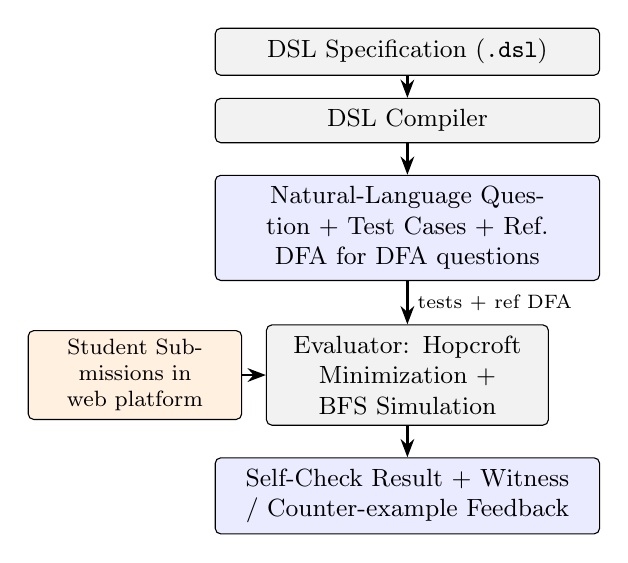
\begin{tikzpicture}[
  box/.style={draw,rounded corners=2pt,fill=gray!10,
    text width=4.6cm,align=center,minimum height=0.5cm,font=\small,inner sep=4pt},
  outbox/.style={draw,rounded corners=2pt,fill=blue!8,
    text width=4.6cm,align=center,minimum height=0.5cm,font=\small,inner sep=4pt},
  subbox/.style={draw,rounded corners=2pt,fill=orange!12,
    text width=2.5cm,align=center,minimum height=0.5cm,font=\footnotesize,inner sep=3pt},
  arr/.style={-Stealth,thick},
  node distance=0.28cm]
\node[box](tpl){DSL Specification (\texttt{.dsl})};
\node [box, below=of tpl](rend){DSL Compiler};
\node[outbox,below=0.4cm of rend](out){Natural-Language Question + Test Cases + Ref.\ DFA for DFA questions };
\node[box,below=0.55cm of out,text width=3.3cm](eval){Evaluator: Hopcroft Minimization + BFS Simulation};
\node[subbox,left=0.3cm of eval](sub){Student Submissions in web platform};
\node[outbox,below=0.4cm of eval](grade){Self-Check Result + Witness / Counter-example Feedback};

\draw[arr](tpl)--(rend);
\draw[arr](rend)--(out);
\draw[arr](out)--(eval) node[midway,right,font=\scriptsize]{tests + ref DFA};
\draw[arr](sub)--(eval);
\draw[arr](eval)--(grade);
\end{tikzpicture}
\caption{AutomataGen pipeline for question generation and self-assessment. The generator (first two stages) synthesizes a unique question, test suite, and reference machine on demand; the evaluator scores each submission against that generated artifact/test suite.}
\label{fig:arch}
\end{figure}

\section{The AutomataGen DSL}

\subsection{The Domain-Specific Language and Instantiation}
Figure~\ref{lst:template} shows a representative DFA specification. An alphabet of size 2 is first sampled from either $\{a,b,c\}$ or $\{0,1\}$; the \texttt{roles} block then binds the abstract role \texttt{A} to the first symbol of that sampled alphabet. The \texttt{parameters} block declares $k$ as a free integer in $[2,6]$, sampled once per instantiation; the \texttt{condition} block is evaluated to synthesize the automaton accepting the described language, and the \texttt{testing} block requests 200 test cases bounded to strings of length 50 or fewer. For example, sampling the window $\{a,b\}$ from $\{a,b,c\}$ (binding role \texttt{A} to \texttt{a}) with $k=6$ resolves \texttt{count(A) \% k == 0} to the natural-language question: \textit{``Construct a DFA over the alphabet $\{a, b\}$ that accepts all strings where the number of `a' symbols is divisible by 6.''} Marking \texttt{closure\_allowed: true} makes this specification eligible to be combined with any other DFA specification over a compatible alphabet under all five closure operations described in Section~\ref{sec:closure}.

\begin{figure}[t]
\centering
\begin{minipage}{0.95\linewidth}
\ttfamily
\begin{tabbing}
AUTOMATA DFA\\
template\_id: DFA\_MOD\_COUNT\\
pattern\_family: \{counting\}\\
difficulty: 1\\
description:\\
\quad Construct a DFA accepting strings where the\\
\quad number of A symbols is divisible by k.\\
alphabet:\\
\quad size: 2\\
\quad symbol\_pools:\{a,b,c\}\\
\quad\qquad\qquad\quad \{0,1\}\\
roles:\{\\
\quad A <- alpha[0]\\
\}\\
parameters:\\
\quad k in [2,6]\\
condition:\\
\quad count(A) \% k == 0\\
testing:\\
\quad cases: 200\\
\quad max\_length: 50\\
tags: \{dfa,counting\}\\
closure\_allowed: true\\
END
\end{tabbing}
\end{minipage}
\caption{Example DSL specification: a modular-counting DFA family.}
\label{lst:template}
\end{figure}

A DSL specification is a plain-text \texttt{.dsl} file declaring: the target machine type (DFA/PDA/TM); an alphabet drawn from one of several symbol pools; role bindings (e.g.\ \texttt{A <- alpha[0]}) that keep specifications alphabet-agnostic; free parameters sampled from declared ranges; a conjunction of conditions built from counting, length, ordering, and string-predicate primitives (e.g. \texttt{prefix\_count(A) >= prefix\_count(B)}, \texttt{palindrome}); and a testing block specifying how many test cases to synthesize and the maximum string length. At generation time the system samples a symbol window and parameter values, solves any free-variable inequalities (e.g.\ $M < N < P$) so that a consistent concrete instance exists within the length budget, and renders a natural-language question. The current specification library spans 55 DSL specifications (17 DFA, 16 PDA, 22 TM) covering pattern families such as modular counting, decimal-equivalent constraints, block ordering, balanced-bracket/Dyck conditions, and palindromes, at author-declared difficulty levels 0--5.

\subsection{Closure-Property Generation and Validation}
\label{sec:closure}

\subsubsection{Class-Aware Structural Derivation}
A primary novelty of \textit{AutomataGen} is its ability to bypass manual authoring through the automated application of closure properties. Given instantiated base questions $q_1$ and $q_2$ over the same alphabet, the system synthesizes fundamentally new state-machine topologies by applying formal operations: Union ($L_1 \cup L_2$), Intersection ($L_1 \cap L_2$), Difference ($L_1 \setminus L_2$), Complement ($\overline{L_1}$), and Reversal ($L_1^R$). From $n$ base specifications, this mechanism combinatorially yields up to $3\binom{n}{2} + 2n$ structurally distinct problems without requiring any additional authoring effort; distinctness itself is enforced by the same session-level \textit{require\_distinguishable} guard (Section~\ref{sec:guards}) applied uniformly to base and closure-derived instances alike.

Crucially, the derivation engine is strict regarding formal language hierarchy boundaries. While regular languages (DFAs and NFAs) and recursive languages (TMs) support all five operations, the generator mathematically restricts context-free languages (PDAs) to Union and Reversal, explicitly preventing the generation of non-CFL problems via intersection or complementation --- properties under which the CFL class is not closed. Furthermore, the system natively implements a construction by using a cross-class closure theorem: given a Regular-language base question $q_{\text{DFA}}$ and a Context-Free base question $q_{\text{PDA}}$ over the same alphabet, it derives a new PDA problem for $L_{\text{DFA}} \cap L_{\text{PDA}}$, since $L_{\text{CFL}} \cap L_{\text{Regular}}$ is context-free. This cross-machine construction is sampled alongside the within-class operations and is capped at 30\% of the requested closure budget, keeping the derived-question mix representative of all five operations rather than dominated by the cross-class case.

\subsubsection{Reference Construction and Validation}
Each derived question is backed by a compositional reference construction: Boolean operations are realized as a product automaton over the two base machines' state sets, and reversal reverses transitions and swaps the start/accept role, keeping DFA-family (and DFA-involving cross-class) closure questions exactly equivalence-checkable via the same Hopcroft-minimization pipeline used for base questions. Derived questions pass back through the four quality guards from Section~\ref{sec:guards}, so a closure operation that collapses to a trivial or empty language is discarded rather than surfaced. A specification may opt out of closure combination entirely via a \texttt{closure\_allowed: false} flag when its combinations would exceed the intended difficulty ceiling.
\subsection{Automatic Quality Guards}
\label{sec:guards}
Generated problems, base or closure-derived, risk being mathematically degenerate --- for example, an intersection that collapses to an empty language ($L_1 \cap L_2 = \emptyset$), or length constraints that leave a condition unsatisfiable within \texttt{max\_length}. To keep instructors free of this burden, every instantiated problem is checked by four automatic guards before being offered to a student, executed in a cheapest-first cascading order that stops at the first failure to save compute cycles: \textit{require\_distinguishable} (checked against a session-level pattern registry to keep every offered problem unique), \textit{require\_non\_empty} ($L \neq \emptyset$ within \texttt{max\_length}), \textit{require\_non\_trivial} ($L \neq \Sigma^*$, ruling out trivial accept-all machines), and \textit{require\_balanced} (at least three ACCEPT and three REJECT strings are reachable, a stricter check than mere non-triviality when \texttt{max\_length} is tight). Problems that fail any guard are discarded and regeneration is retried (up to five times); specifications that still cannot produce a valid instance after retrying are flagged.

\section{On-Demand Practice Workflow}
A student selects a machine type and difficulty tier (easy/medium/ hard, mapped to underlying specification difficulty levels) and requests a problem; the backend filters eligible specifications, instantiates one live, runs it through the quality guards, and---depending on machine type---attaches a small set of public example strings distinct from the hidden grading test cases plus, for DFA, a reference automaton for equivalence checking.

Figure~\ref{fig:practice-ui} shows the practice interface for a generated DFA question. The left panel displays the natural-language question text, the sampled alphabet ($\{b,c\}$), the length bound, and a small set of public example test cases (labelled ACCEPT/REJECT) distinct from the hidden grading suite; the main canvas is a JFLAP-style construction surface where the student builds their automaton interactively.

\begin{figure*}[t]
\centering
\includegraphics[width=0.55\textwidth]{ondemand-cropped.png}
\caption{The on-demand practice interface: a generated DFA question (modular-counting family, $k=5$) with its natural-language description, sampled alphabet, public example test cases, and the interactive construction canvas.}
\label{fig:practice-ui}
\end{figure*}

\section{Technical Evaluation}

Because AutomataGen has not yet been deployed to a live cohort, we evaluate the pipeline's reliability and scale rather than learning outcomes, requesting five instances per specification across all 55 specifications and 20 closure-derived questions end-to-end, with results in Table~\ref{tab:eval}.

\begin{table}[t]
  \caption{Generation pipeline: technical evaluation}
  \label{tab:eval}
  \small
  \setlength{\tabcolsep}{3pt}
  \begin{tabular}{p{3.7cm}p{1.4cm}p{1.5cm}}
    \toprule
    \textbf{Metric} & \textbf{Value} & \textbf{Notes}\\
    \midrule
    DSL specifications authored & 55 & 17 DFA, 16 PDA, 22 TM \\
    Base instances requested & 275 & 5 $\times$ 55 specifications \\
    Base instances passing all guards & 232 (84.4\%) & auto-retried \\
    Closure questions requested & 20 & 5 op.\ types \\
    Closure questions produced & 16 (80.0\%) & \\
    \bottomrule
  \end{tabular}
\end{table}

The 84.4\% first-pass guard rate confirms the guards are doing real work---roughly one instance in six 
is discarded rather than shipped as an empty, trivial, or duplicate problem---while the pipeline completes 
each request within seconds, the latency needed for live, on-demand use. 
The run's 295 instances (275 base plus 20 closure-derived) already exceed the volume a 
single 30-student practice session would generate at one request per student, 
so the demonstrated throughput comfortably covers cohorts of that size. 
Table~\ref{tab:compare} compares against the two most closely related systems from Section~\ref{sec:related-work}.

\begin{table}[t]
  \caption{Comparison with JFLAP and Automata Tutor}
  \label{tab:compare}
  \small
  \setlength{\tabcolsep}{3pt}
  \begin{tabular}{p{2.05cm}p{1.25cm}p{1.65cm}p{1.4cm}}
    \toprule
    \textbf{Capability} & \textbf{JFLAP} & \textbf{Automata Tutor} & \textbf{AutomataGen}\\
    \midrule
    Construction or  & Yes & Yes & Yes\\
    simulation UI     &    &     &    \\
    Auto.\ problem generation & No & DFA only & DFA, PDA, TM\\
    Per-question test cases & No & Internal & Yes, tunable\\
    Closure-derived variants & No & No & Yes\\
    \bottomrule
  \end{tabular}
\end{table}

\section{Discussion and Conclusion}
AutomataGen is intended for deployment in an undergraduate automata theory practical course, 
replacing a fixed problem sheet with session-based, non-repeating practice across DFA, PDA, and TM construction; 
we have not yet collected classroom data on learning outcomes, engagement, or instructor workload. 
Known limitations include: specification authoring requires DSL familiarity, and supporting a new condition operator requires extending the DSL Compiler (lexer, parser, and AST) rather than being expressible within existing specifications. We plan to (i) run a semester-long deployment with usage and outcome data, and (ii) explore automatic DSL specification authoring assistance to lower the barrier for new instructors.

We presented AutomataGen, a DSL-driven web platform for automata theory practice that generates 
two kinds of questions on demand: base questions instantiated directly from instructor-authored DSL specifications, 
and class-aware closure-derived questions formed by combining pairs of instantiated specifications under union, intersection, difference, complement, and reversal, with four automatic quality guards validating the semantic well-formedness of every generated question, across DFA, PDA, and Turing machines. 
Each question, base or closure-derived, carries a machine-synthesized test suite, and DFA-family questions additionally carry a reference automaton enabling exact, equivalence-based self-checking; PDA and TM questions are self-checked against their generated test cases. The platform is live at \url{https://automata-gen.onrender.com/practice}, 
and its full source, including all 55 DSL specifications, is publicly available under the MIT license at \url{https://github.com/venkyjntu-git/AutomataGen}.

\begin{acks}
Portions of this manuscript's prose and parts of the AutomataGen implementation were developed with the assistance of Claude (Anthropic); the authors reviewed all AI-assisted content and take full responsibility for its accuracy.
\end{acks}

\bibliography{references}

\end{document}
